\begin{frame}[c]{}
\begin{center}
    \textbf{Part III: A Stronger Assumption: The (Strong) Exponential Time Hypothesis}
    
    \textit{Proving Lower Bounds for Subexponential Time}
\end{center}
\end{frame}


\begin{frame}[c]{Why We Need a New a Assumption}

\begin{center}
We already know for the \textbf{Vertex Cover} problem:

\begin{enumerate}
    \pause\item $2^n \cdot \mathrm{poly}(n)$ by brute-forcing all sets
    \pause\item $2^k \cdot \mathrm{poly}(n)$ by \textit{branching} (Introduction)
\end{enumerate}

But for example: \textbf{Planar Vertex Cover} can be solved in 

\\~

\begin{enumerate}
    \pause\item $2^{\mathcal{O}(\sqrt{n})}$ by a given Tree-Decomposition + Dynamic Programming \footnote{Because $tw(G)\leq\sqrt{n}$ for planar G. Recent 2-Approximation Algorithm see (\cite{twapprox})}
\end{enumerate}
\end{center}

\end{frame}
\begin{frame}[c]{Fine-Grained Complexity}

\textbf{Sad News:} The fundamental assumption $\mathbf{P \neq NP}$ rules out all attempts for finding a PTIME algorithm for NP-c problems.
\\~

\pause\textbf{Question}: Can we at least \textbf{hope} for a \textit{Sub-Exponential} Time Algorithm for NP-Complete problems? 

\pause\begin{center}
  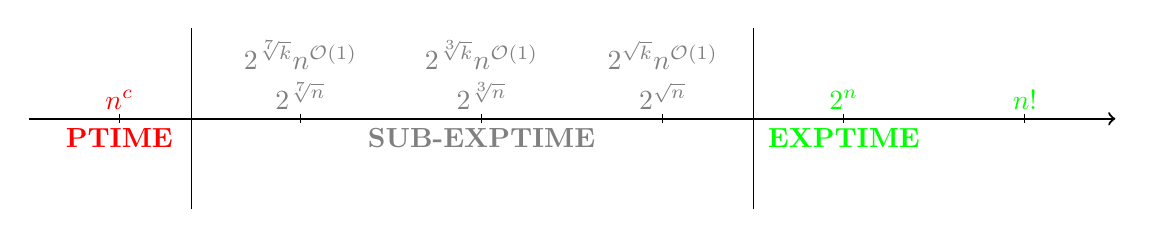
\begin{tikzpicture}[scale=1.15]
  \draw[thick, ->] (0,0) -- (12,0) node [below] {};
    \foreach \x in {1,3,...,12}
    \draw (\x, 0.05) -- node[pos=0.5] (point\x) {} (\x, -0.05);
    %\draw (\x, 0.1) -- node[pos=0.5] (point\x) {} (\x, -0.1);
    % node's content --- access them as point1...point5
    \path (point1) node [red, below] {\textbf{PTIME}};
    \draw (1.8, -1) -- node[pos=0.5] (point2) {} (1.8, 1);
    %\draw (\x, 0.1) -- node[pos=0.5] (point\x) {} (\x, -0.1);
    \path (point1) node [red, above] {\textbf{$n^c$}};
    %\path (point1) node [above] {$A=1$};
   \path (point3) node [gray, above] {\textbf{$2^{\sqrt[7]{n}}$}};
   \path (point3) node [gray, above=0.5cm] {\textbf{$2^{\sqrt[7]{k}} n^{\mathcal{O}(1)}$}};
    \path (point5) node [gray, above] {\textbf{$2^{\sqrt[3]{n}}$}};
    \path (point5) node [gray, above=0.5cm] {\textbf{$2^{\sqrt[3]{k}} n^{\mathcal{O}(1)}$}};
   %\path (point5) node [gray, above] {\textbf{$2^{\log(n)}$}};
    \path (point5) node [gray, below] {\textbf{SUB-EXPTIME}};
    \path (point7) node [gray, above] {\textbf{$2^{\sqrt{n}}$}};
    \path (point7) node [gray, above=0.5cm] {\textbf{$2^{\sqrt{k}} n^{\mathcal{O}(1)}$}};
    \path (point9) node [green, above] {\textbf{$2^{n}$}};
    \path (point11) node [green, above] {\textbf{$n!$}};
    \draw (8, -1) -- node[pos=0.5] (point8) {} (8, 1);
    \path (point9) node [green, below] {\textbf{EXPTIME}};
  \end{tikzpicture}
\end{center}

\pause\textbf{Solution}: A new assumption based again on the \textit{Hardness of SAT} 

\end{frame}

\begin{frame}[c]{ETH and SETH}
    \begin{exampleblock}{Exponential Time Hypothesis}
        There is $\delta > 0$ s.t. $\mathtt{3SAT}$ can not be solved in time $\mathcal{O}(2^{\delta n}) = \mathcal{O}((2^{\delta})^n)$ 
    \end{exampleblock}
    
    \pause\begin{exampleblock}{Strong Exponential Time Hypothesis}
        For every $\delta < 1$ there is $q$ s.t. $\mathtt{qSAT}$ cannot be solved in time $\mathcal{O}(2^{\delta n})$
    \end{exampleblock}
    
    %q-SAT inevitabily getting more difficult
    
\begin{enumerate}
%    \item $2^{\delta n} = (2^\delta)^n$: $\exists$ no algorithm solving 3SAT in $\mathcal{O}(\delta^n)$ with $\delta \leq 1$ 
    \pause\item $\mathtt{ETH} \Rightarrow \mathtt{3SAT}$ can not beat $2^{\mathcal{O}(n)}$ 
    \pause\item $\mathtt{SETH} \Rightarrow \mathtt{ETH}$ (Proof: \cite[Theorem 14.5]{Cygan2015})
    \pause\item  $\mathtt{ETH}$ is commonly believed, $\mathtt{SETH}$ still discussed.
\end{enumerate}
\end{frame}

\begin{frame}[c]{Transfering Lower Bounds by Reductions}

Observe the \textbf{Textbook} reduction (e.g. \cite{redvc}) from $\mathtt{3SAT} \leq \mathtt{VERTEX~COVER}$:

\\~

For example given: $ \phi = (x \lor y \lor \overline{z}) \land (x \lor \overline{y}) \land (\overline{x} \lor \overline{z} \lore \overline{y})$
    \begin{center}
        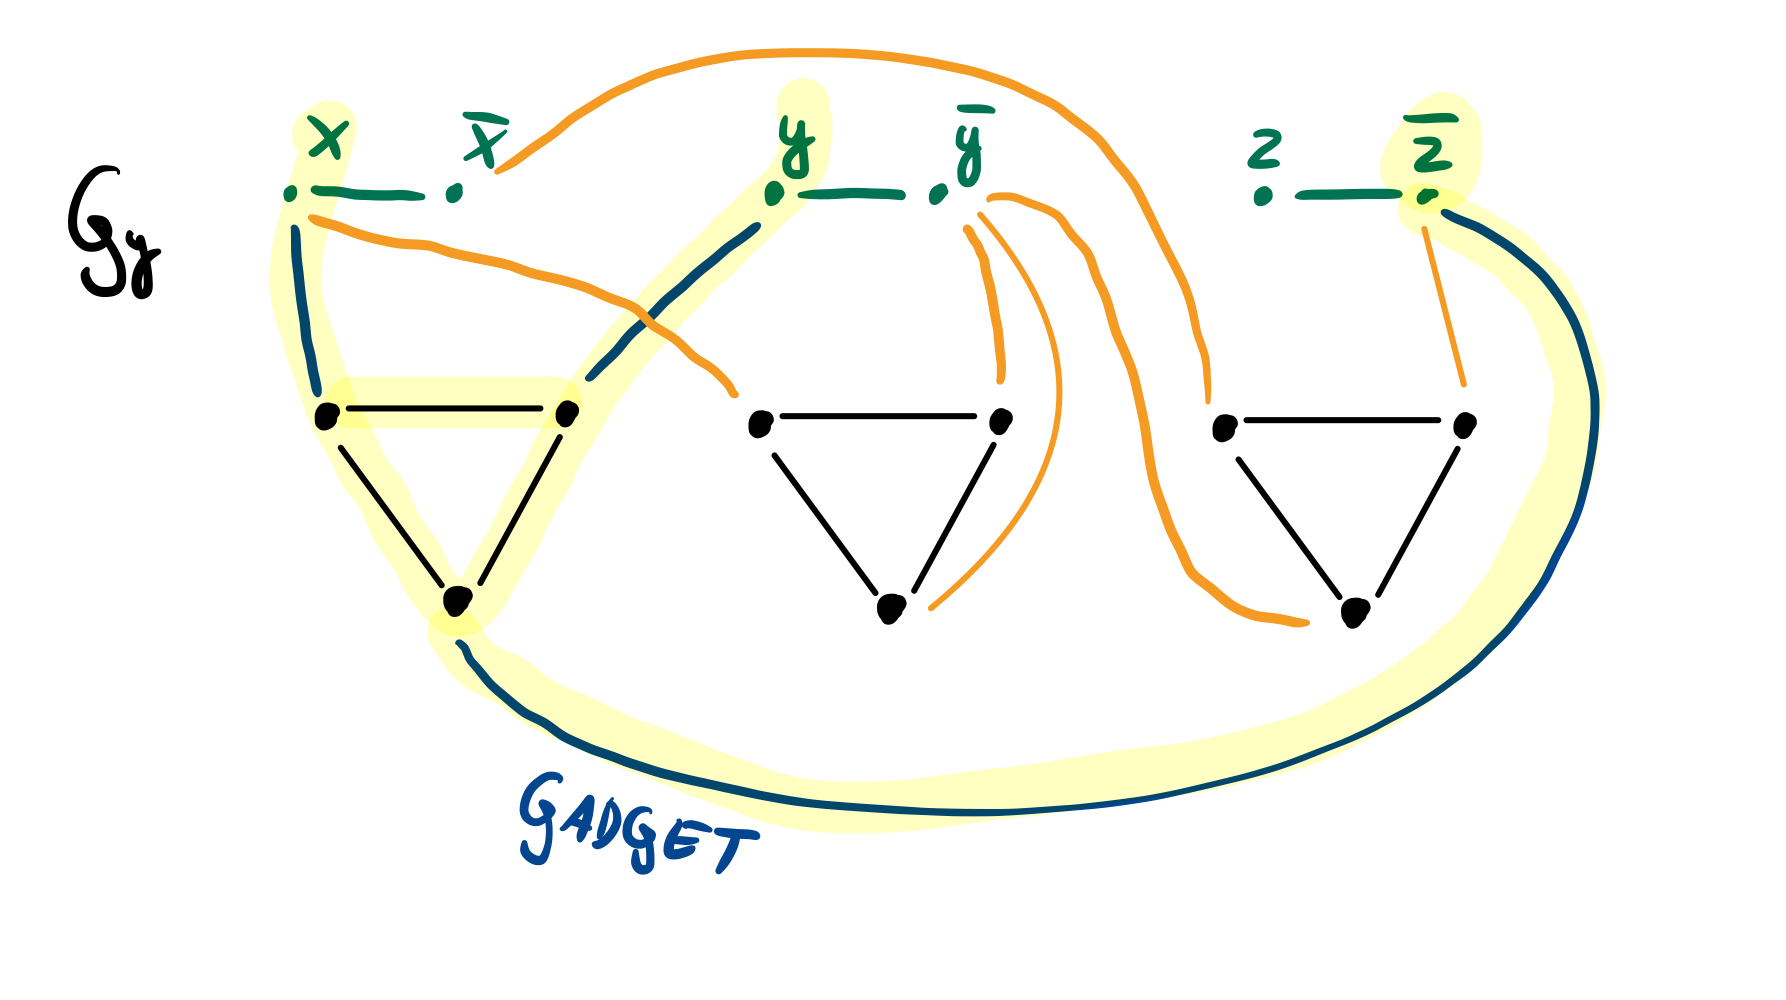
\includegraphics[scale=0.12]{img/reduce-to-VC.png}
    \end{center}
    
%\begin{block}{Observation 1}
%       Simmons Hall is composed of metal and concrete.
%\end{block} %   \begin{alertblock}{Observation 1}
\end{frame}

\begin{frame}[c]{$\mathtt{3SAT} \leq \mathtt{VERTEX~COVER}$: Analysis}
\begin{center}

$\begin{bmatrix}
   \text{Formula~} \phi \\
   n \mathtt{~Variables} \\
   m \mathtt{~Clauses} \\
\end{bmatrix} \rightsquigarrow	
\begin{bmatrix}
   \text (G, k)\\
   2n + 3m \mathtt{~Vertices} \\
   n + 6m \mathtt{~Edges} \\
   k = 2n + m
\end{bmatrix} 
$

\begin{itemize}
       \item $\#\mathtt{clauses}_{\mathtt{3SAT}} = m = \binom{2N}{3} \in \mathcal{O}(n^3)$
       \item $\Rightarrow$ size of the whole instance $N,M \in \mathcal{O}(n^3)$
\end{itemize}
      
\pause\begin{block}{Corollary}
Assume $\mathtt{VERTEX~COVER}$ can be solved in time $2^{o(\sqrt[3]{N+M})}$

$\Rightarrow \mathtt{3SAT}$ could be solved in $2^{o(n)}$ by \textit{pipelining} the reduction. \textbf{\textcolor{red}{\text{\faBolt}}}
 Contradicting ETH
 
\end{block}

\\~ 
\begin{center}
    \pause\textbf{Nice. But can we do better?}
\end{center}
\\~ 
\end{center}
\end{frame}

\begin{frame}[c]{Towards a Tight Bound: Sparsification Lemma}

\textbf{Idea: }If we tighten $m = \mathcal{O}(n)$ in the input instance, then we would get $2^{o(N+M)}$ by the same (linear) reduction

\begin{block}{Outlook: Sparsification Lemma (\cite{sparslem})}{
For all $\epsilon > 0$, there is a constant $K$ s.t. we can compute for every formula $\phi$ in $\mathtt{3CNF}$ with $n$ clauses over $k$ variables an equivalent formula $\bigvee_{t=1}^t \psi_i$ where each $\psi_i$ is in $\mathtt{3CNF}$ and over the same $k$ variables and has $\leq K \cdot k$ clauses. Moreover, $t \leq 2^{\epsilon k}$ and the computation takes $\mathcal{O}(2^{\epsilon k}n^c)$ time
}
\end{block}
\textbf{Proof: } Omitted, but idea: Branching over a set of variables.
\end{frame}

\begin{frame}[c]{Sketch: Turning Back to Our Reduction}
\begin{enumerate}
    \item Using \textbf{Sparsification Lemma} we can \textit{sparsify} our kCNF-formula to \textbf{linear size} in clauses with an appropriate $\epsilon$.
    \item We apply our reduction from $\mathtt{3SAT} \leq \mathtt{VERTEX~COVER}$
    \item Total Runtime now lowerly bounded by $2^{o(N + M)}$  
\end{enumerate}
\end{frame}

\begin{frame}[c]{More Tight Bounds For Classical Problems}

\textbf{Consequence: } Assuming ETH, there is no $2^{o(n)}$ time algorithm for

\\~
\begin{center}

\begin{itemize}
    \item $\mathtt{INDEPENDENT~SET}$
    \item $\mathtt{CLIQUE}$
    \item $\mathtt{DOMINATING~SET}$
    \item $\mathtt{VERTEX~COVER}$
    \item $\mathtt{HAMILTONIAN~PATH}$
    \item $\mathtt{FEEDBACK~VERTEX~SET}$
\end{itemize}

\end{center}
\end{frame}
\begin{frame}[c]{Crucial Consequence for FPT Algorithms}

\textbf{Observation: } No $2^{o(n)}$-Time Algorithm $\Rightarrow$ also no $2^{o(k)} \cdot n^{\mathcal{O}(1)}$-Time Algorithm
\\~

\textbf{Consequence: } Assuming ETH, there is no $2^{o(k)} \cdot n^{\mathcal{O}(1)}$ time algorithm for

\\~
\begin{center}

\begin{itemize}
    \item \textcolor{red}{k-}$\mathtt{INDEPENDENT~SET}$
    \item \textcolor{red}{k-}$\mathtt{CLIQUE}$
    \item \textcolor{red}{k-}$\mathtt{DOMINATING~SET}$
    \item \textcolor{red}{k-}$\mathtt{VERTEX~COVER}$
    \item \textcolor{red}{k-}$\mathtt{HAMILTONIAN~PATH}$
    \item \textcolor{red}{k-}$\mathtt{FEEDBACK~VERTEX~SET}$
\end{itemize}

\end{center}
\end{frame}

\begin{frame}[c]{Last Slide: Lower Bounds for $\omega[1]$ hard problems}

We can even go further:

\begin{block}{Theorem \cite{clique}}Assuming ETH, there is no $f(k) \cdot n^{o(k)}$ algorithm for $\mathtt{CLIQUE}_k$ for any computable function $f$
\end{block}

Implying that we can not have \textbf{any FPT algorithms} for
\begin{itemize}
    \item $\mathtt{SET~COVER}$, $\mathtt{HITTING~SET}$, $\mathtt{CONNECTED~DOMINATING~SET}$, $\mathtt{PARTIAL~VERTEX~COVER}$, $\mathtt{...}$
\end{itemize}
unless ETH fails.

This closes the cycle back to our $\omega[i]$-hierarchy.

\end{frame}
%\begin{frame}[c]{Consequences For Parametrized Problems}
%http://cs.bme.hu/~dmarx/papers/marx-simons3.pdf
%Asuming ETH no FPT  w hard
%Because ... this instantly rules out fpt.-.. for particulat
% TODO tight bounds for parametrized problems as well

%\textbf{In General: } If there is a PTIME reduction from $\mathtt{3SAT} \leq_{\mathtt{FPT}} L$, where $k \leq f(n+m)$, then assuming ETH \textbf{L cannot be solved in time $2^{o(f^{-1}(k))}\cdot poly(|x|)$}
%\end{frame}

\begin{frame}[c]{Key Takeaways III}
\begin{center}
\begin{quote}
    If there would be just three things, you should take away...
\end{quote}
\begin{itemize}

\item ETH: $\exists \delta > 0$ s.t. $\mathtt{3SAT}$ can not be solved in time $\mathcal{O}(2^{\delta n })$
\item Lower Bounds (under ETH) can be transferred using reductions
\item That I thank all of you very much for the attention!
\end{itemize}
\end{center}
\end{frame}
